\section{Analysis}

\begin{figure}[t]
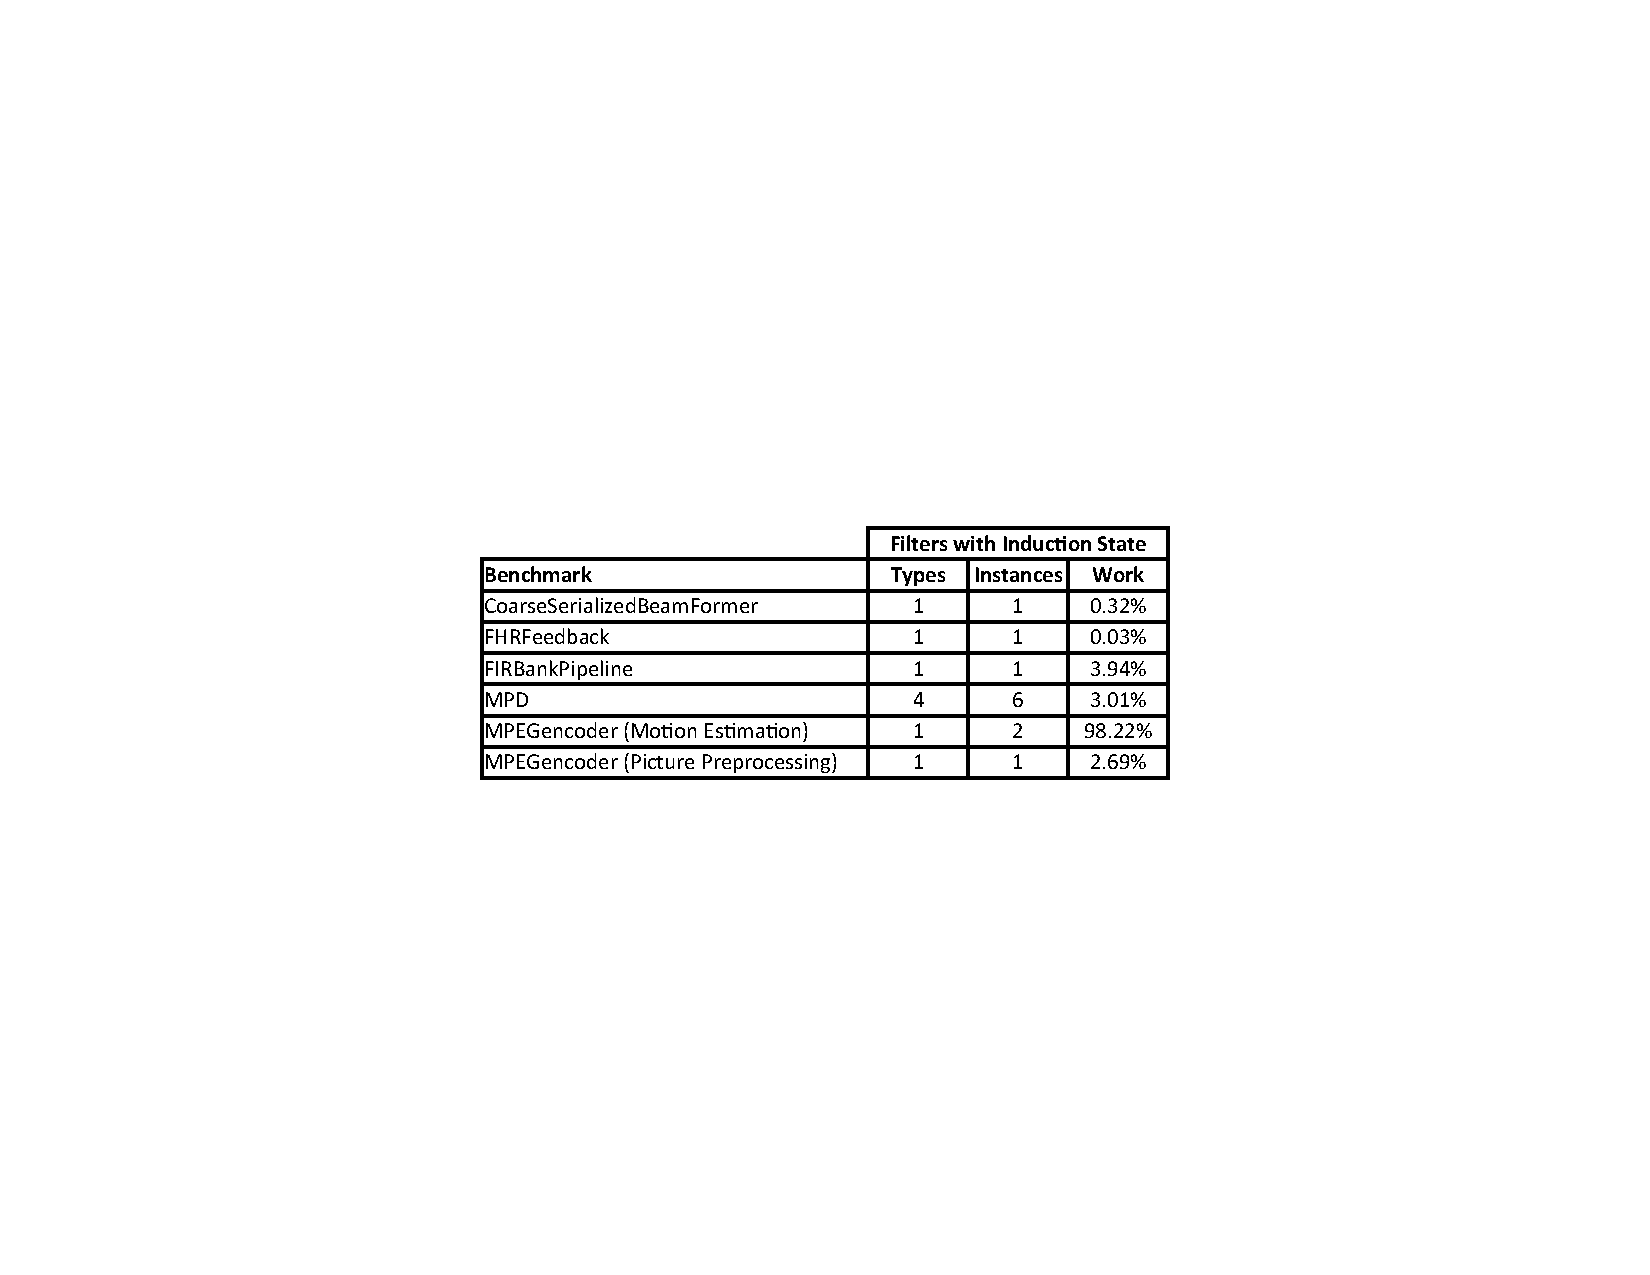
\includegraphics[width=3.3in]{figures/induction-benchmarks.pdf}
\caption{Benchmarks using induction variable state and estimations on work performed in filters with induction state.\protect\label{fig:benchmarks}}
\end{figure}

Figure~\ref{fig:benchmarks} indicates programs in the StreamIt benchmark suite that use induction variable filters (not including source filters).  The StreamIt compiler provides static estimations of work performed in filters.  The above table indicates the work performed in specifically the induction variable filters.

The majority of programs do not have substantial work performed in filters using induction variables, the MPEG-2 motion estimation subset being the exception.  However, eliminating state will have a large impact on runtime performance even on programs with low work concentration in stateful filters.  We model the potential speedups of a particular stateful program in this section.  For the purpose of this analysis, we will assume no communication cost between filters.  We will also assume the compiler exposes no pipeline parallelism.  This assumption forces the serialization of stateful filters on the stream graph.

Let $N$ be the number of cores we are planning to parallelize over.  Let $\sigma$ be the percentage of work performed in stateful filters that can have its state eliminated, in this case solely filters that use induction variable state.  

If $\sigma = 0$, the entire program is stateless.  The program can be fused to coarsen the granularity, then fissed and mapped to all of the available cores.  Each core would perform $\frac{1}{N}$ of the total work.  Thus with no state, the program can exhibit speedups of up to $N$ times the single-core runtime.

For filters that contain stateful work, we describe the program in terms of work that can be parallelized with work that cannot be parallelized.  $1-\sigma$ of the work in the program is considered stateless, and thus can be fissed and assigned to $N$ individual cores.  The stateful filters cannot be parallelized, and is sequential to all work in the program.  The total serialized work is $\frac{1-\sigma}{N} + \sigma$.  Thus the total speedup is the amount of work done without parallelization, or 100\% of the work, divided by the new parallelized work.  
\begin{eqnarray*}
\dfrac{1}{\frac{1-\sigma}{N} + \sigma} &=& \dfrac{N}{1 + \sigma(N-1)}
\end{eqnarray*}

We can characterize the amount of speedup between a completely stateless program to an equivalent stateful program with $\sigma$ percentage of stateful work.  This is simply:
\begin{eqnarray*}
\dfrac{N}{\frac{N}{1 + \sigma(N-1)}} &=& 1 + \sigma(N-1)
\end{eqnarray*}



\begin{figure}[t!]
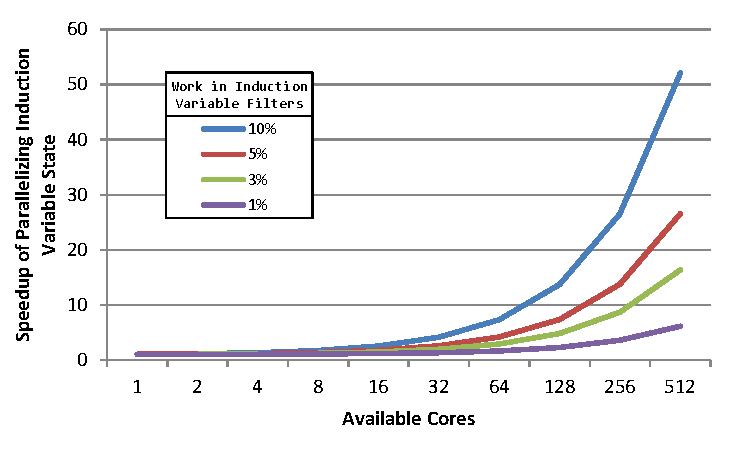
\includegraphics[width=3.3in]{figures/theoretic-speedup.pdf}
\caption{Theoretical speedups for stateless filters over corresponding stateful filters with $\sigma$\% work.  \protect\label{fig:theo-speedups}}
\end{figure}

Figure~\ref{fig:theo-speedups} indicates the potential speedups over stateful programs given stateful work percentages and a varying number of cores.  Even benchmarks in the suite that exhibit only 3\% work in stateful filters can exhibit 8x speedups with 256 cores.  Providing a means to remove state from filters that exhibit very small amounts of work relative to the rest of the program can still generate substantial speedups in the near future.



\begin{figure}[t]
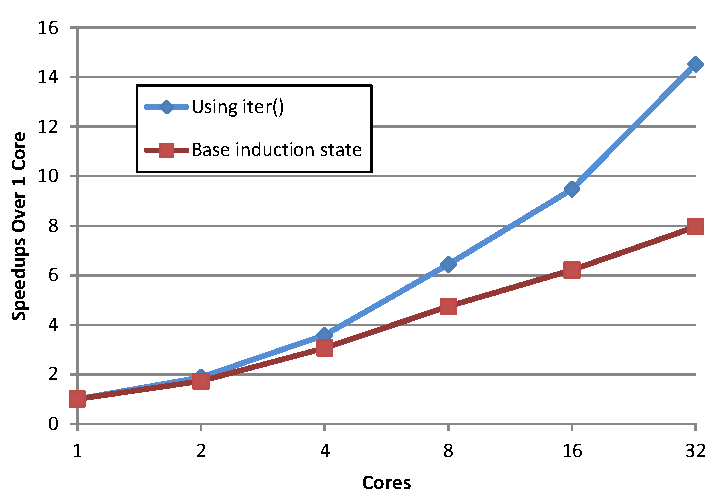
\includegraphics[width=3.3in]{figures/firbank-results.pdf}
\caption{Speedups for FIRBankPipeline, with and without induction variable state.  \protect\label{fig:firbank-results}}
\end{figure}

FIRBankPipeline contains one filter that uses induction variable state.  According to Figure~\ref{fig:benchmarks}, there is 3.94\% of work performed in the induction filter, which represents the only state in this benchmark.  Figure~\ref{fig:firbank-results} indicates the speedups over 1 core for both stateful and stateless implementations.  Between stateful and stateless implementations, there is 1.35X speedup on 8 cores, 1.58X speedup on 16 cores, and 1.84X speedup on 32 cores, which abides fairly closely to the model.